
\documentclass[a4j,10pt,onecolumn,oneside,titlepage,final]{jarticle}
% 図をFig. に変えておく
\renewcommand{\figurename}{Fig.}

%%%%%%%%%%%%%%%%%%%%%%%%%%%%%%%%%%
% 以下必要に応じて執筆先にコピペ

% 画像
\usepackage[dvipdfmx]{graphicx}
% リンク
\usepackage[dvipdfmx]{hyperref}
% 目次
\usepackage{pxjahyper}
% フォント関連
\usepackage{amsfonts}
\usepackage{amsmath, amssymb}
\usepackage{mathrsfs}	% for \mathscr{}
\usepackage{bm}
% 図や表の引用
\newcommand{\figref}[1]{Fig.\,\ref{#1}}
\newcommand{\Figref}[1]{Figure\,\ref{#1}}
\newcommand{\figsref}[2]{Figs.\,\ref{#1} -- \ref{#2}}
\newcommand{\Figsref}[2]{Figures\,\ref{#1} -- \ref{#2}}
\newcommand{\tabref}[1]{Table\,\ref{#1}}
% 数式記号
\newcommand{\tp}{\mathsf{T}}	% tp: transpose
\newcommand{\sgn}{\operatorname{sgn}}
\newcommand{\argmin}{\mathop{\rm arg~min}\limits}
% Theorem 関連
% 日本語
\usepackage{amsthm}
\theoremstyle{definition}
\newtheorem{definition}{定義}
\newtheorem{theorem}[definition]{定理}
\newtheorem{proposition}[definition]{命題}
\newtheorem{remark}[definition]{注意}
\renewcommand\proofname{\bf 証明}

\setlength{\topmargin}{0pt}
\iftombow{}
\addtolength{\topmargin}{-1in}
\else
\addtolength{\topmargin}{-1truein}
\fi
\setlength{\textheight}{26cm}
\setlength{\textwidth}{17cm}
\setlength{\oddsidemargin}{-0.5cm}
% % English
% \newtheorem{definition}{Definition}
% \newtheorem{theorem}[definition]{Theorem}
% \newtheorem{lemma}[definition]{Lemma}
% \newtheorem{corollary}[definition]{Corollary}
% \newtheorem{proposition}[definition]{Proposition}
% \newtheorem{remark}[definition]{Remark}
% \newtheorem{example}[definition]{Example}

%%%%%%%%%%%%%%%%%%%%%%%%%%%%%%%%%%

\begin{document}
\twocolumn[
\begin{flushright}令和a年b月c日(金)\end{flushright}
\begin{center}\LARGE\bf{班名}\end{center}
\begin{center}\LARGE\bf{週報 第d回\\週報タイトル \\ ここにタイトル}
\end{center}\large
\vspace*{2mm}
{\Large \begin{flushright}
岩瀬 研究室~~~学番 ~\\ 名前\\
%学番と名前を書いたら「学籍番号,氏名」は消してください
指導教員  岩瀬~将美 教授
\end{flushright}}]

%\inputで章ごとに作成も可能
% pdfにしおりをつけたくないときはsection*{}にする
\section{To Do List}	
	\begin{itemize}
	\item{やること1}
		\begin{itemize}
			\item 論文調査 
		\end{itemize}
	\item {やること2}
		\begin{itemize}
			\item{詳細書く}
		\end{itemize}
	\end{itemize}

\newpage

\section{前回の週報内容}
	\begin{itemize}
	\item{内容}
	\end{itemize}
	
\section{今回の研究概要}
	\begin{itemize}
		\item{論文調査}
	\end{itemize}

\section{今後の予定}
	\begin{itemize}
		\item{内容1}
		\item{内容2}
		\begin{itemize}
			\item{詳細書く}
			\item{詳細書く}
		\end{itemize}
	\end{itemize}

	\section{備考(適宜タイトル変更もしくは追加)}
	\begin{itemize}
		\item{内容1}
		\item{内容2}
		\item {内容3}
		\item {内容4}
	\end{itemize}
\newpage
\section{テンプレの説明}
これは,岩瀬研究室用のvscode対応週報テンプレです.
出力はoutに格納されています.
図はfig内に格納して参照してください.
参考文献はbibtex(reference)に対応しています\cite{1}
reserch.texには具体的な研究内容を書いてください.
週報以外でvscodeを使いたい場合はフォルダにそれ用のstyファイルとtexファイルを追加してください.
ATACSテンプレなどは動作確認済み.\\
分からないことがあればhttps://github.com/sige0002を参照してください.



\section{1章}
chapterでファイルを小分けにできます.
画像はこのように表示できます.
\begin{figure}[tbp]
  \centering
  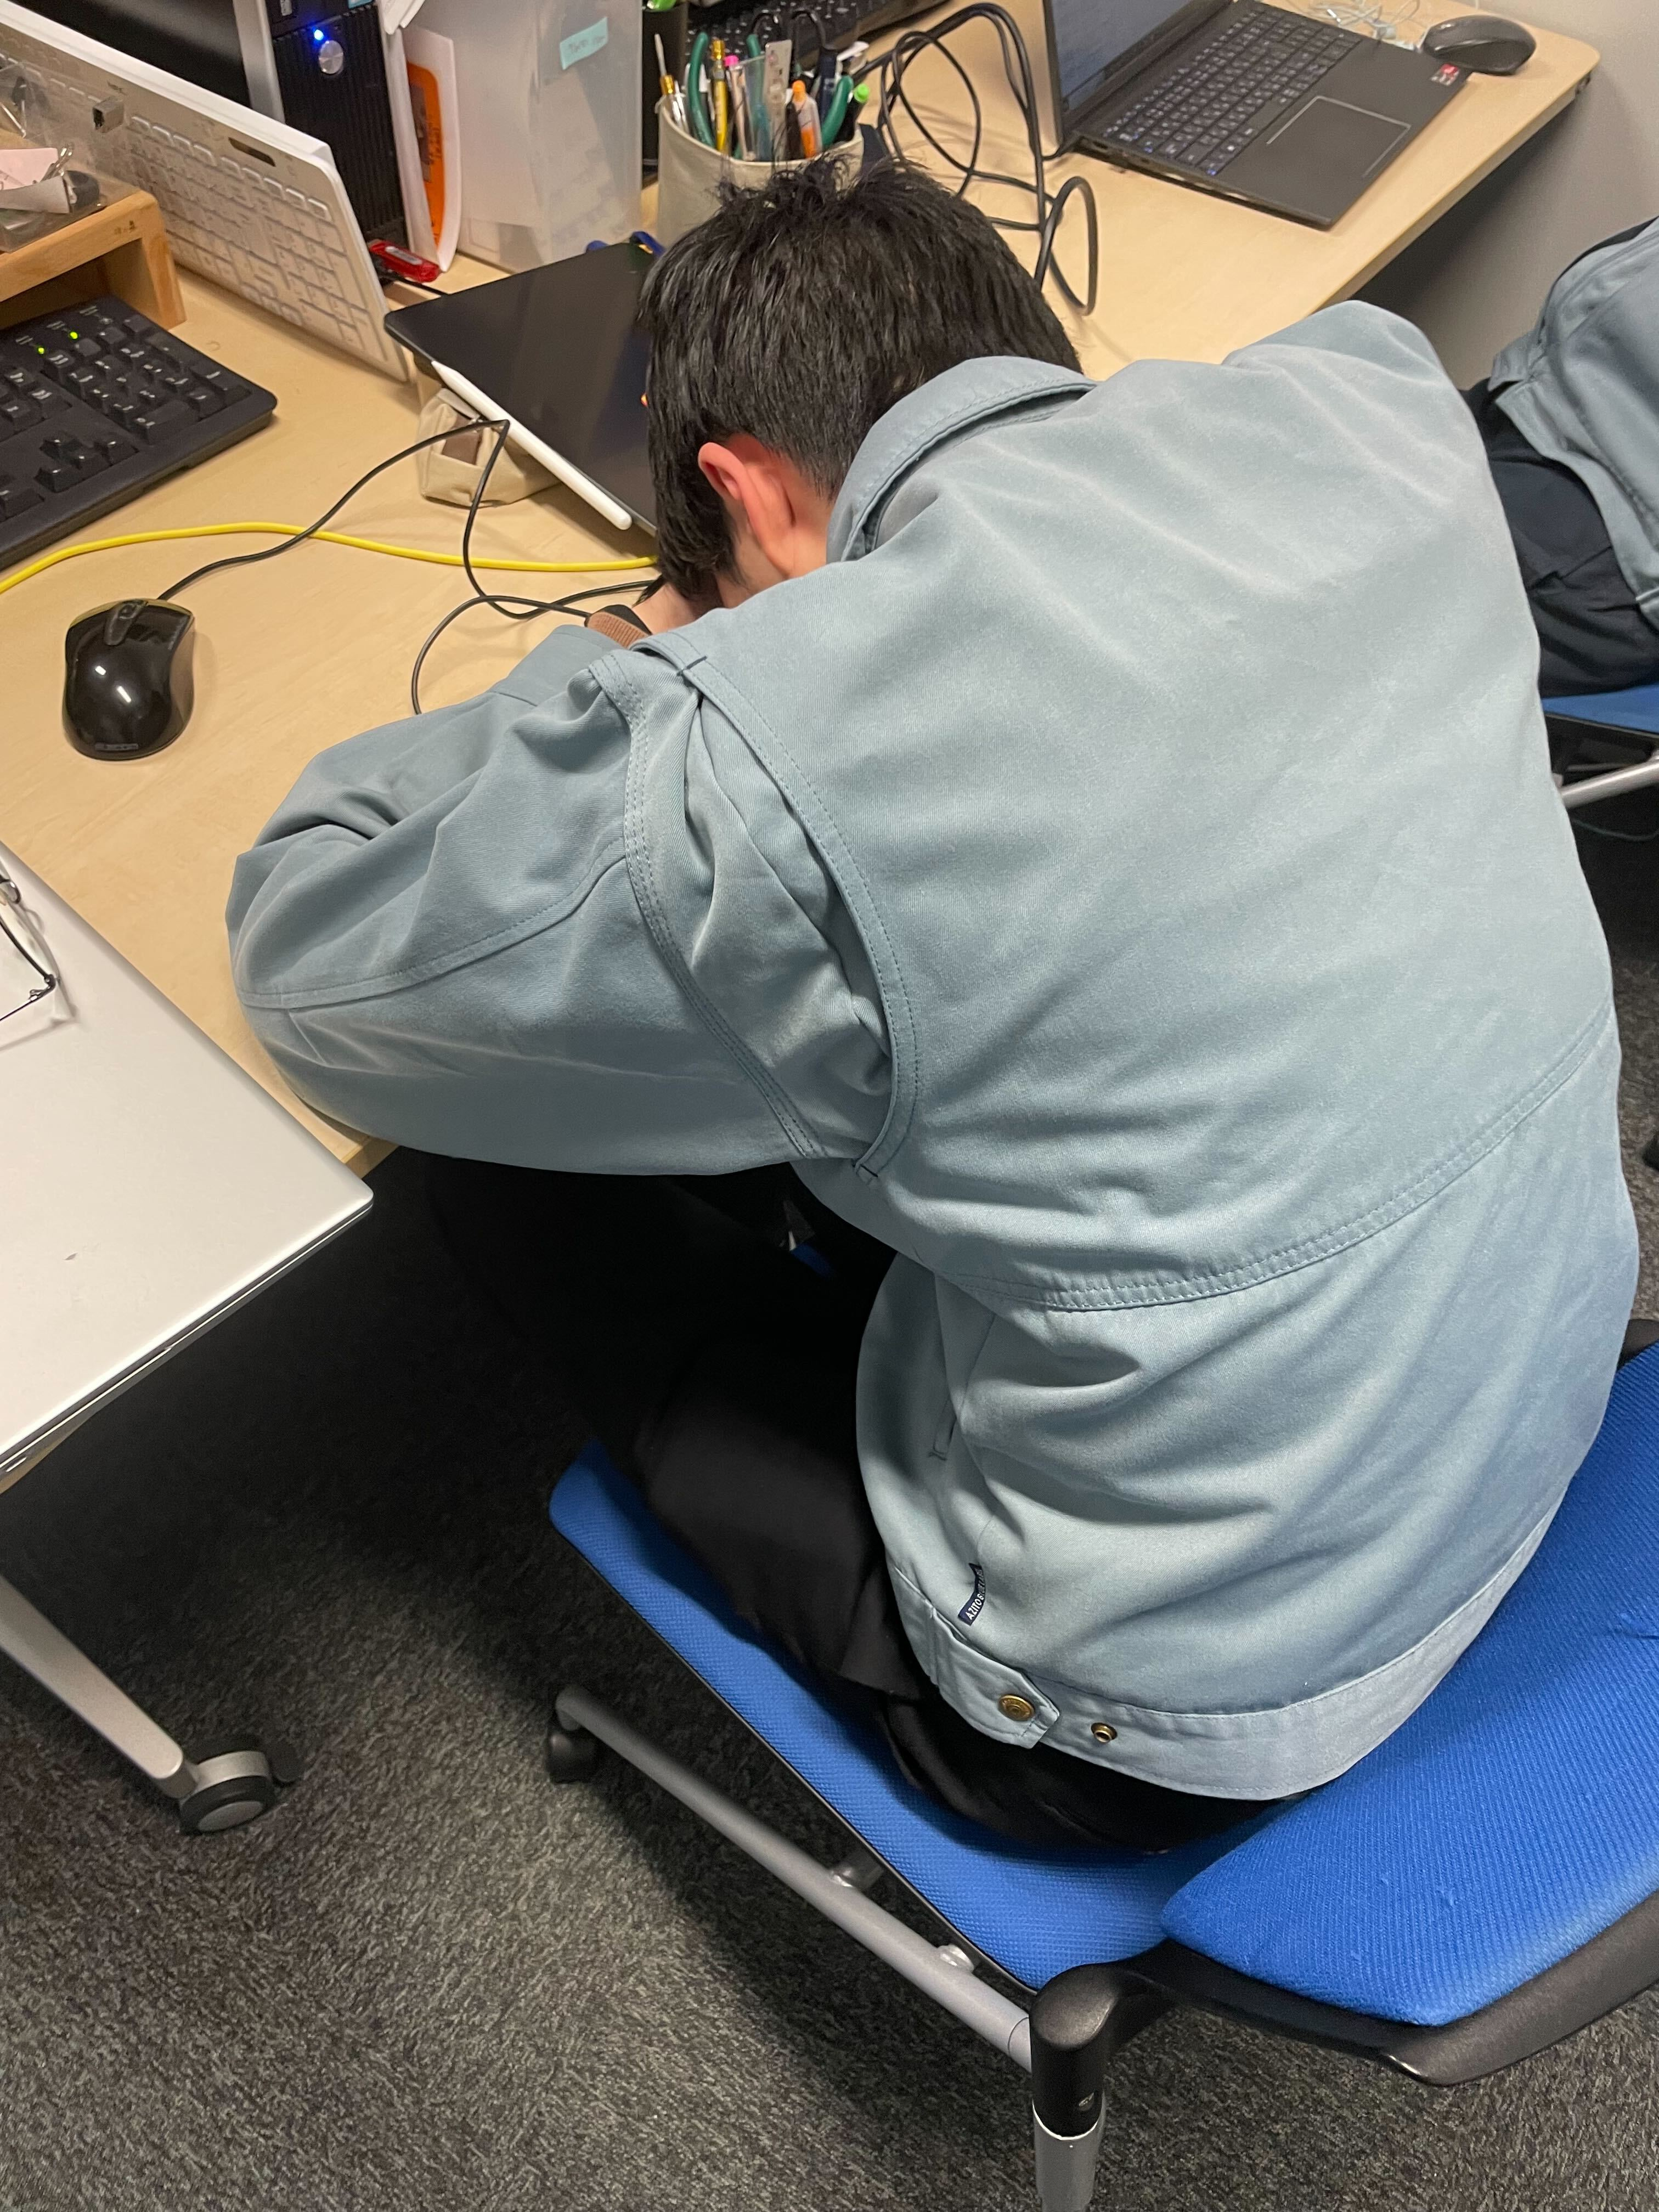
\includegraphics[width=7cm]{./fig/酒井_サボり.eps}
  \vspace{-5pt}
  \caption{サンプル画像}
  \label{fig:sample}
  \end{figure}

\bibliographystyle{junsrt}
\bibliography{reference} % reference.bib を読み込む
% \nocite{*} % 引用がされていないものも表示する
\end{document}
